\section{Results}\label{sec:validation}
This section applies the particle model to two prescribed baths. The
Faner experiment compares solvent loading and temperature with source
readings; the DT experiment follows the coupled solvent, moisture and
thermal response of a particle from feed to exit. Both use the same
particle conservation laws, phase equilibrium, retention closures and
reference transport coefficients; their gas histories, geometry and
initial states differ. Liquid-water imbibition operates when an external
water film contacts the dry shell.

\subsection{Falling-rate drying in Faner's superheated-hexane experiment}
\label{sec:validation:journalmarch}\label{sec:validation:fanermarch}
\label{sec:validation:faner}\label{sec:validation:hexanebp}\label{sec:results:lumpedlaw}
\paragraph{Experimental basis and declared particle.}
The soybean run of \citet{faner2019kinetics} supplies pure n-hexane vapour
at \SI{120}{\celsius} and atmospheric pressure. The article explicitly
reports preheating inside the apparatus and no visible warming-up stage.
It does not specify the exact initial temperature. Its product-temperature
trace initially lies near the reported \SI{68.7}{\celsius} boiling plateau.
We therefore use a uniform initial body at the calculated pure-hexane
boiling temperature, \SI{68.8}{\celsius}, as a declared approximation to
that plateau, rather than a measured preheat endpoint.
Initial loadings are $X_{\mathrm h}=0.475$ and $X_{\mathrm w}=0.0250$
kg/kg dry meal, with oil mass fraction 0.0195. Initial moisture is unreported;
the positive water loading is a study input that keeps water active in the
shared model, rather than a measured property of Faner's charge.
The flakes were desolventized in nitrogen, crumbled and stored at ambient
conditions before being re-embedded in hexane. Their initial water therefore
cannot be inferred directly from fresh extractor meal moisture.
Water loss was not reported separately, so interpreting the gravimetric
mass loss as hexane removal introduces an additional observable uncertainty.

The source's image analysis gives a mean equivalent-sphere diameter of
\SI{1.77}{\milli\metre}, mean sphericity 0.74, an overall diameter range
0.5--4 mm and 95.1\% of soybean particles between 1 and 3 mm. These
summaries do not specify a mass-weighted size histogram. The complete
trajectory uses the reported mean diameter directly, giving a spherical
radius of \SI{0.885}{\milli\metre}. This choice anchors the particle size
to the experiment without adjusting it to the drying curve.
It preserves equivalent volume rather than flake shape: a sphere has less
surface per volume than a flake of the reported sphericity. The alternative
surface-to-volume radius, $0.74\times1.77/2=0.655$ mm, preserves that area
ratio but does not reproduce the flake's internal transport distances.
Neither mapping reconstructs the unreported mass-weighted size distribution.
A truncated lognormal construction consistent with the source summaries
is documented in Sec.~\ref*{S-sup:journalensemble}; its previous reduced
trajectories do not supply the current particle results.

\paragraph{Heat supply and shared model.}
The film exposure multiplier, 0.146, scales both gas-side heat and mass
transfer coefficients while leaving the spherical area unchanged. It was
identified from the heat duty implied by Faner's early constant-rate
solvent loss, using an earlier particle-size ensemble, and was not
reidentified for the present sphere. The digitized source readings and
the calculation are given in Sec.~\ref*{S-sup:fanermultiplier}.
The unscaled coefficients describe
an industrial reference gas flow, whereas Faner's apparatus uses a thin
sample layer, approximately three to five particle diameters deep
\citep{faner2019kinetics}. The multiplier therefore specifies an effective
experimental boundary; it is not a measured exposed-area fraction.
Scaling mass transfer by the same factor is an additional boundary
assumption, since the early heat duty does not identify it independently.
The resulting heat coefficient is 15.1 W/(m$^2$ K), compared with
104 W/(m$^2$ K) before scaling. Thus the early constant-rate agreement
involves boundary calibration; the falling-rate and temperature comparisons
are conditional on that boundary, with the particle coefficients held fixed.
Faner also inferred heat transfer coefficients from experimental drying
data \citep{faner2019kinetics}.

For the four separate 2008 thesis runs, Whitaker's packed-bed correlation predicts
0.82--1.06 times the measured constant-rate duty on the wet-charge
mass convention, whereas reading the charge as dry meal gives
0.53--0.61. Two inferred coefficients lie 3.7\% and 4.2\% below the
correlation. These checks concern external supply rather than an
independent identification of intraparticle transport
(Sec.~\ref*{S-sup:filmmatch}).
An otherwise unchanged calculation with multiplier one exhausts external
free hexane at 6.8 s, compared with 46.8 s in the reported calculation.
This early-stage sensitivity demonstrates the importance of the gas-side
boundary; it does not establish that the industrial reference coefficients
represent Faner's apparatus (Sec.~\ref*{S-sup:detail:geometry}).
For reference, Faner's geometric comparator is
\begin{equation}
\front=\Rp\left(\frac{\Xh-\Xe}{\Xc-\Xe}\right)^{1/3},
\label{eq:faneroracle}
\end{equation}
where $\Xe$ is that source's equilibrium loading. The present calculation
instead solves the component and energy jumps; Eq.~\eqref{eq:faneroracle}
is not an additional front constraint.

Both experiments use binary pore diffusivity
$6.0\times10^{-10}$ m$^2$/s, retained-water mobility
$8.47\times10^{-7}$ mol/(m s) and conductivity 0.24 W/(m K).
These coefficients define the common engineering case; they are not
independently identified by the two experiments. Holding them fixed makes
the comparison a test of the same transport description in different baths.
The positive-water Luikov
continuation described in Section~\ref{sec:model:dry} is used throughout.
In regime A, external free hexane is assumed to isolate retained water
from the pure-hexane bath: water exchange is zero while its mass and energy
remain stored. This surface-access approximation is not a measured barrier
property. In regimes B and C, water evolves through the pore-gas and
retained-water equations. Liquid-water imbibition is inactive here because
there is no external water film.

Figure~\ref{fig:journalmarch} compares the four-cell calculation with
Faner's readings on the reported experimental clock. Loading includes
all particle hexane per unit dry meal; temperature is the particle volume
mean, while the thermocouple measures a local holder temperature.
Markers show the measurements with their digitization half-widths. The dotted vapour line is the
prescribed nominal temperature; the dashed line is the measured vapour
trace, shown for comparison. Calculated water and liquid-hexane core volume
are supporting results in Fig.~\ref*{S-fig:fanersupport}.

\begin{figure}[htbp]\centering
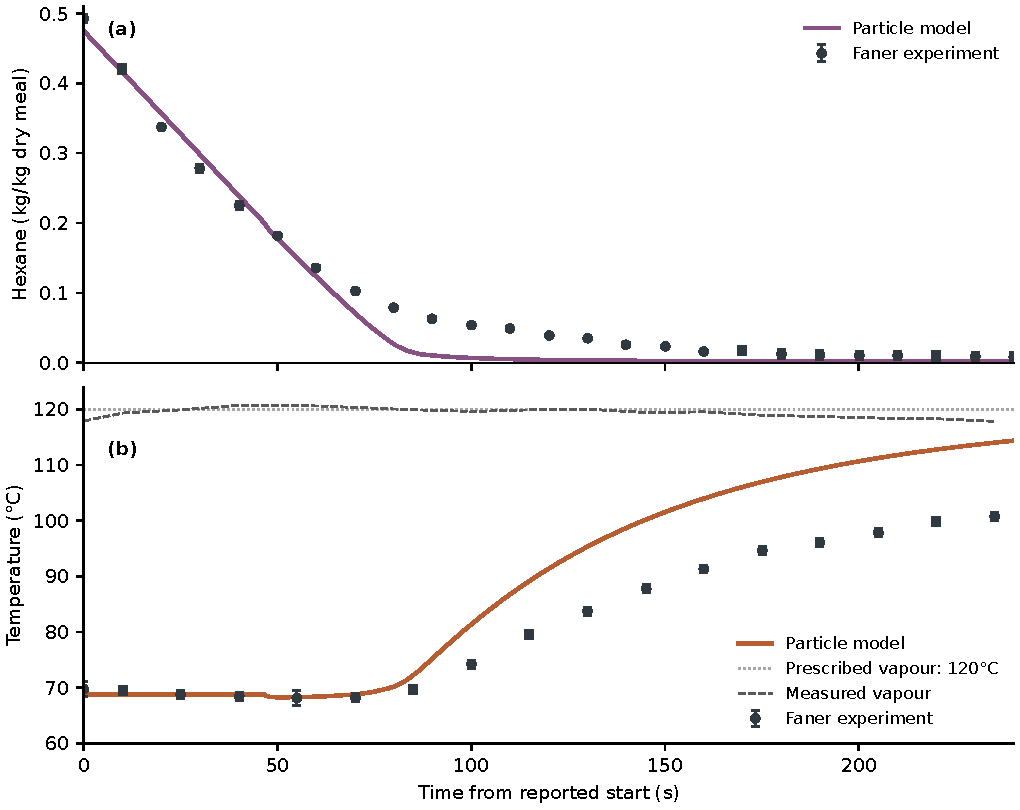
\includegraphics[width=\textwidth]{figures/fig_faner_particle_history_core2.pdf}
\caption{Faner's pure-hexane experiment: (a) hexane loading and
(b) particle temperature. Lines show calculations; markers show measurements.}
\label{fig:journalmarch}
\end{figure}

\paragraph{Solvent removal and temperature.}
External free hexane disappears at \SI{\FanerFreeEnd}{\second}; the core vanishes at
\SI{\FanerDryTime}{\second}. Loading crosses 0.20 kg/kg at
\SI{\FanerCrossTwenty}{\second} and reaches 0.10 kg/kg a further
\SI{\FanerFallingInterval}{\second} later, versus 45.9 s and 25.4 s in
the digitized source. The calculated falling interval is about
\FanerFallingShortfall\% shorter.
At 240 s, hexane is $\FanerExitHexane$ kg/kg dry, water is
$\FanerExitWater$ kg/kg dry and mean temperature is
\SI{\FanerExitTemperature}{\celsius}.
This discrepancy cannot be assigned to one mechanism: the particle sizes
are known only as summaries, the initial moisture is unknown, and the local
exposure and the thermocouple sampling are uncertain.
Table~\ref{tab:journalmarch} summarizes the comparison; loading crossings
are interpolated between successive calculated states. Its temperature
comparison retains the distinction between local holder and particle mean.

\begin{table}[htbp]\centering\small
\caption{Faner comparison on the reported experimental clock.}
\label{tab:journalmarch}
\begin{tabular}{@{}lrr@{}}\toprule
Observable & Faner experiment & Particle model\\\midrule
Time to $X_{\mathrm h}=0.20$, s & 45.9 & \FanerCrossTwenty\\
Interval $0.20\to0.10$, s & 25.4 & \FanerFallingInterval\\
Liquid-core disappearance, s & Not measured & \FanerDryTime\\
Water at 240 s, kg/kg dry & Not reported & \FanerExitWater\\
Temperature at 235.1 s, $^\circ$C & 100.8 & \FanerLastHolderClockTemperature\\
\bottomrule\end{tabular}\end{table}

Using the reported mean diameter instead of the smaller sphere inherited
from earlier calculations delays removal and warming: the external area per dry mass decreases and
the internal transport distances increase. This improves the loading
crossing while leaving a falling-rate discrepancy. At matched four-cell
resolution, the 80--100$^\circ$C temperature milestones occur about
12--17 s later than with the inherited smaller sphere. In a DT heat balance,
that timing determines how long the heat supply goes mainly to evaporation
before the meal warms, affecting residence requirements and product quality.
The source-mean two-cell march loses its core at 90.1 s; the four-cell
value is \SI{\FanerDryTime}{\second}. Their positive-core step sequences
also differ, so this comparison is a resolution sensitivity rather than
a continuum limit.

The measured vapour varies from 117.8 to \SI{120.7}{\celsius}, rather than
remaining exactly at its nominal value. A separate two-cell sensitivity
applies that trace after core depletion and gives \SI{113.0}{\celsius}
at 240 s, compared with \SI{114.3}{\celsius} under constant vapour
temperature. The small improvement supports treating heat-supply
variation as an experimental uncertainty; it does not close the full
temperature discrepancy. Before core depletion, this sensitivity still
uses the nominal bath (Sec.~\ref*{S-sup:fanerassumptions}).
Startup calculations at higher initial moisture, 0.050 and 0.100 kg/kg,
are not yet resolved (Sec.~\ref*{S-sup:journalmarch}).

\subsection{Particle destiny in the prescribed DT bath}
\label{sec:validation:dtmarch}\label{sec:validation:otherchecks}
\label{sec:validation:uptake}\label{sec:validation:tail}\label{sec:validation:bp}
\label{sec:validation:envelope}\label{sec:validation:rewetting}\label{sec:validation:derived}
\paragraph{Bath and initial state.}
The DT experiment uses an effective spherical radius $\Rp=\SI{1.5}{\milli\metre}$
and follows the particle from feed to the prescribed exit at
\SI{1766.5}{\second} (29.4 min). This radius is the coarse end of the
previous size screening. It is consistent with the upper end of the
0.5--1.5-mm equivalent-radius range containing 95.1\% of Faner's soybean
particles \citep{faner2019kinetics}, but is not a measured DT mean.
The longer heat path and smaller surface area per unit mass make this a
useful coarse-particle case when examining residence needed for solvent
removal. It does not represent a mass-weighted meal size distribution.

Initial temperature is \SI{49.0}{\celsius}, hexane and water loadings are
0.388 and 0.124 kg/kg dry meal, and oil mass fraction is 0.0137.
The feed is cooler than the 57--60$^\circ$C examples reported by
\citet{witte_nd_soybeanmeal} and \citet{kemper2013solvent}, so sensible
heating remains part of this experiment. The selected temperature is a
scenario input, rather than a measurement for the simulated charge.
The pre-desolventizing (PD) bath is at \SI{72.0}{\celsius} with hexane mole
fraction 0.664, exposure fraction 0.00408 and indirect heat supply
85 W/kg dry until \SI{490.2}{\second}. Steam contact then leads to a
toasting bath ending at \SI{105.0}{\celsius}. The prescribed gas history
is detailed in Sec.~\ref*{S-sup:dtmarch}.

The sequence represents indirect pre-desolventizing followed by live-steam
contact, as described by \citet{kemper2013solvent}. Indirect heating removes
solvent before steam contact and reduces the solvent load on the
steam-heated trays. The selected exposure fraction approximates the small
exposed area of a bed compared with the summed areas of isolated spheres.
This exposure fraction, the imposed duty and the bath ladder together
define the experiment; they do not identify a measured industrial
operating point.
Liquid-water imbibition uses the closure of
Section~\ref{sec:model:liquidcontact}, with liquid contact conductance
0.32 mol/(m$^2$ s), derived from the uptake time of solvent-extracted meal
in liquid water, and total dry-shell retained-water mobility 1000 times
the reference retained-water mobility, the water-filled-pore limit. Both inputs were set
before and independently of the DT outlet.

\paragraph{Liquid depletion, condensation and imbibition.}
At PD exit, about 0.169 kg external free hexane/kg dry remains. It disappears
approximately 2.1 s later while the external water film accumulates.
The initial two-liquid surface equilibrium is near \SI{61.3}{\celsius};
it differs from pure hexane's boiling point. The dry shell forms at
492.3 s and core extinction occurs at 503.6 s, approximately 11.3 s after
external free-hexane depletion. Retained hexane and pore gas then
continue to evolve in regime C. Both the rapid surface evaporation and the
core recession follow from the coupled balances.

At core extinction, the particle contains 0.136 kg water/kg dry and the
external water film contains a further 0.086 kg/kg dry. The film remains
until 624.5 s, about two minutes after dry-shell formation. Liquid-water
imbibition and evaporation back to the bath compete for this inventory;
condensation does not imply that all incoming water remains in the particle.
The external water film supplies mass and energy for several minutes and
persists into regime C.

Figure~\ref{fig:dtmarch} presents wet-basis hexane and moisture alongside
the volume-mean particle temperature. Dashed curves use the right axes
for the prescribed bath mole fractions and temperature. The lower
timeline identifies pre-desolventizing and main trays; dotted vertical
lines mark A--B and B--C. The insets resolve the brief core recession
and the external water film. Green markers at 30 min show published
outlet ranges: 16--22\% moisture from Witte and 100--500 ppm solvent
and 105--110$^\circ$C temperature from Kemper
\citep{kemper2013solvent,witte_nd_soybeanmeal}. They provide industrial
context rather than paired measurements of this prescribed bath.
The calculated history ends at 29.4 min.

\begin{figure}[htbp]\centering
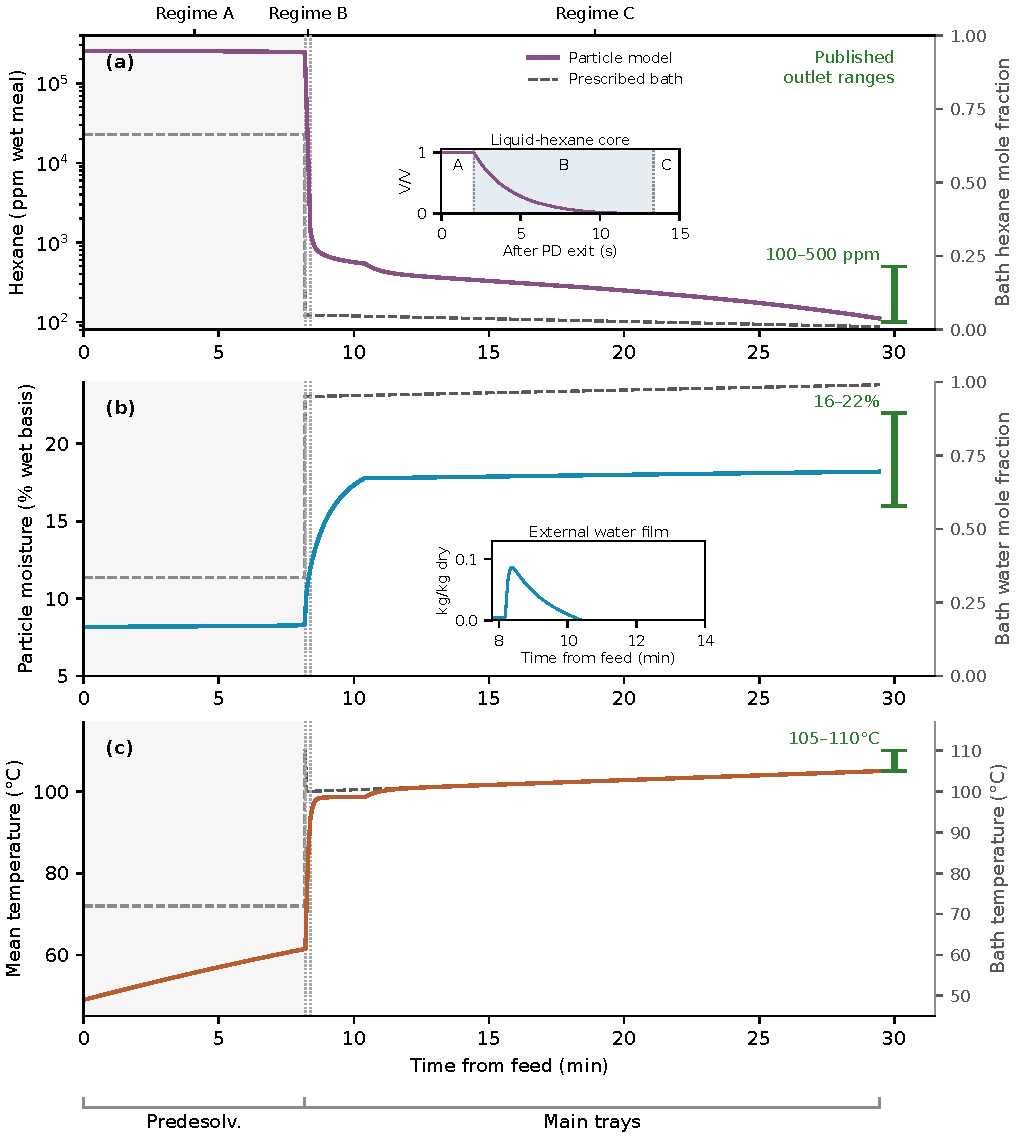
\includegraphics[width=\textwidth]{figures/fig_dt_particle_history_core2.pdf}
\caption{DT particle destiny: (a) hexane, (b) moisture and (c) temperature.
Solid lines show the particle response; dashed lines show the bath.
Green markers indicate published outlet ranges.}
\label{fig:dtmarch}
\end{figure}

\paragraph{Exit observables and numerical sensitivity.}
Particle water at exit is 0.223 kg/kg dry meal, equivalent to 18.2\%
wet-basis moisture. Hexane is 135 mg/kg dry, or 111 ppm on a wet basis, and
volume-mean particle temperature is \SI{105.0}{\celsius}.
The external water film is depleted. The particle-only basis conversion
uses $1+X_{\mathrm w}+X_{\mathrm h}$; water in the external water film is reported
separately while the film is present.
Table~\ref{tab:dtmarch} compares the result with the published outlet
ranges. Calculated ppm uses wet meal; the source solvent range does not
specify its analytical mass basis. The calculation uses two radial cells
and a 5-s maximum regime-C timestep.

\begin{table}[htbp]\centering\small
\caption{DT exit results and published outlet ranges.}
\label{tab:dtmarch}
\begin{tabular}{@{}lrl@{}}\toprule
Observable & Particle model & Published range\\\midrule
Hexane, mg/kg dry & 135 & Mass basis not specified\\
Hexane, ppm wet & 111 & 100--500\\
Particle moisture, \% wet & 18.2 & 16--22\\
Volume-mean temperature, $^\circ$C & 105.0 & 105--110\\
External water film, kg/kg dry & 0 & Not measured\\
\bottomrule\end{tabular}\end{table}

The calculated outlet lies within the published ranges. This agreement
cannot identify the imbibition coefficients or validate the prescribed bath.
In the reference case at $K_\ell=0.10$ mol/(m$^2$ s), halving the
regime-C maximum timestep from 10 to 5 s changes moisture by
0.022 percentage points, hexane by 0.52\%, temperature by 0.0016 K and
water-film depletion time by 1.8 s. The regime-B history is unchanged in
this check; full-history mesh convergence is not yet established
(Section~\ref{sec:discussion:limits}).
An independent reconstruction of every accepted advance from dry-shell
formation to exit gives maximum normalized water, hexane and energy
defects of $4.24\times10^{-11}$, $8.61\times10^{-13}$ and
$6.16\times10^{-12}$, respectively. The earlier feed audit is retained separately. The coupled
result closes the stated balances; the material transport rates
remain to be identified independently.
